
\chapter{Introduzione}
L'obiettivo del progetto realizzato è quello di integrare la libreria OROCOS KDL (\url{https://www.orocos.org/kdl.html}) nel component framework \textit{STAR} per definire un'applicazione che consente di inviare al robot comandi di posizione della pinza montata all'estremità del robot manipolatore P-Rob 3 (\Fig\ref{fig:prob3}) rispetto al sistema di riferimento cartesiano alla base del robot.
\begin{figure}[b!]
	\centering
	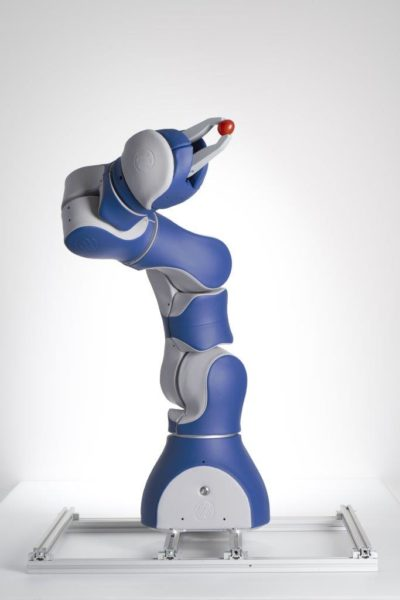
\includegraphics[width=0.4\linewidth]{./ImageFiles/P-Rob 3.jpg}
	\caption{Robot manipolatore P-Rob 3.}
	\label{fig:prob3}
\end{figure}
In particolare, si sono sviluppate le seguenti funzionalità:
\begin{itemize}
	\item calcolo della posizione della pinza rispetto al sistema di riferimento alla base del robot a partire dal valore degli angoli dei giunti (cinematica diretta);
	\item calcolo del valore dei giunti a partire dalla posizione della pinza rispetto al sistema di riferimento alla base del robot (cinematica inversa);
	\item calcolo di un percorso lineare a partire da una posizione iniziale e una finale della pinza.
\end{itemize}

\chapter{Libreria OROCOS KDL}
\section{Definizione del modello del robot}
Per realizzare i calcoli cinematici si è scelto di utilizzare la libreria OROCOS KDL, che implementa le funzionalità base come il calcolo della cinematica diretta e inversa di un robot. Seguendo la guida di installazione disponibile nella documentazione (\url{https://www.orocos.org/wiki/Installation_Manual.html}), la libreria è stata integrata nel framework \textit{STAR} al seguente percorso: STAR/AutonomousRobot/Libraries/others/orocos\_kinematics\_dynamics. Inoltre, per semplificare alcune operazioni di inizializzazione della libreria, è stato integrato anche un kdl parser nel percorso STAR/AutonomousRobot/Libraries/others/kdl\_parser, seguendo le istruzioni di installazione reperibili al seguente link \url{STAR/AutonomousRobot/Libraries/others/orocos\_kinematics\_dynamics}. 

Per effettuare i calcoli cinematici, la libreria ha bisogno di conoscere la struttura del robot. La catena cinematica del robot è definita in modo standard in un file .urdf (\url{http://wiki.ros.org/urdf}), nel quale sono descritti tutti i parametri, quali ad esempio il numero, la tipologia e i limiti dei giunti e la lunghezza dei link. Per definire questo file, si è partiti dal modello fornito sulla pagina github del produttore (\url{https://github.com/fp-robotics/fp_descriptions}), seguendo la procedura per la generazione dell'urdf. Successivamente, il file descrittore definitivo è stato definito estrapolando le informazioni rilevanti per il progetto e, eseguendo delle prove con l'interfaccia web fornita dal produttore del robot, sono stati verificati alcuni dati presenti nell'urdf. La catena cinematica descritta dall'urdf è riportata in figura \ref{fig:urdf_prob3}.

\newpage
\begin{figure}[tbh]
	\centering
	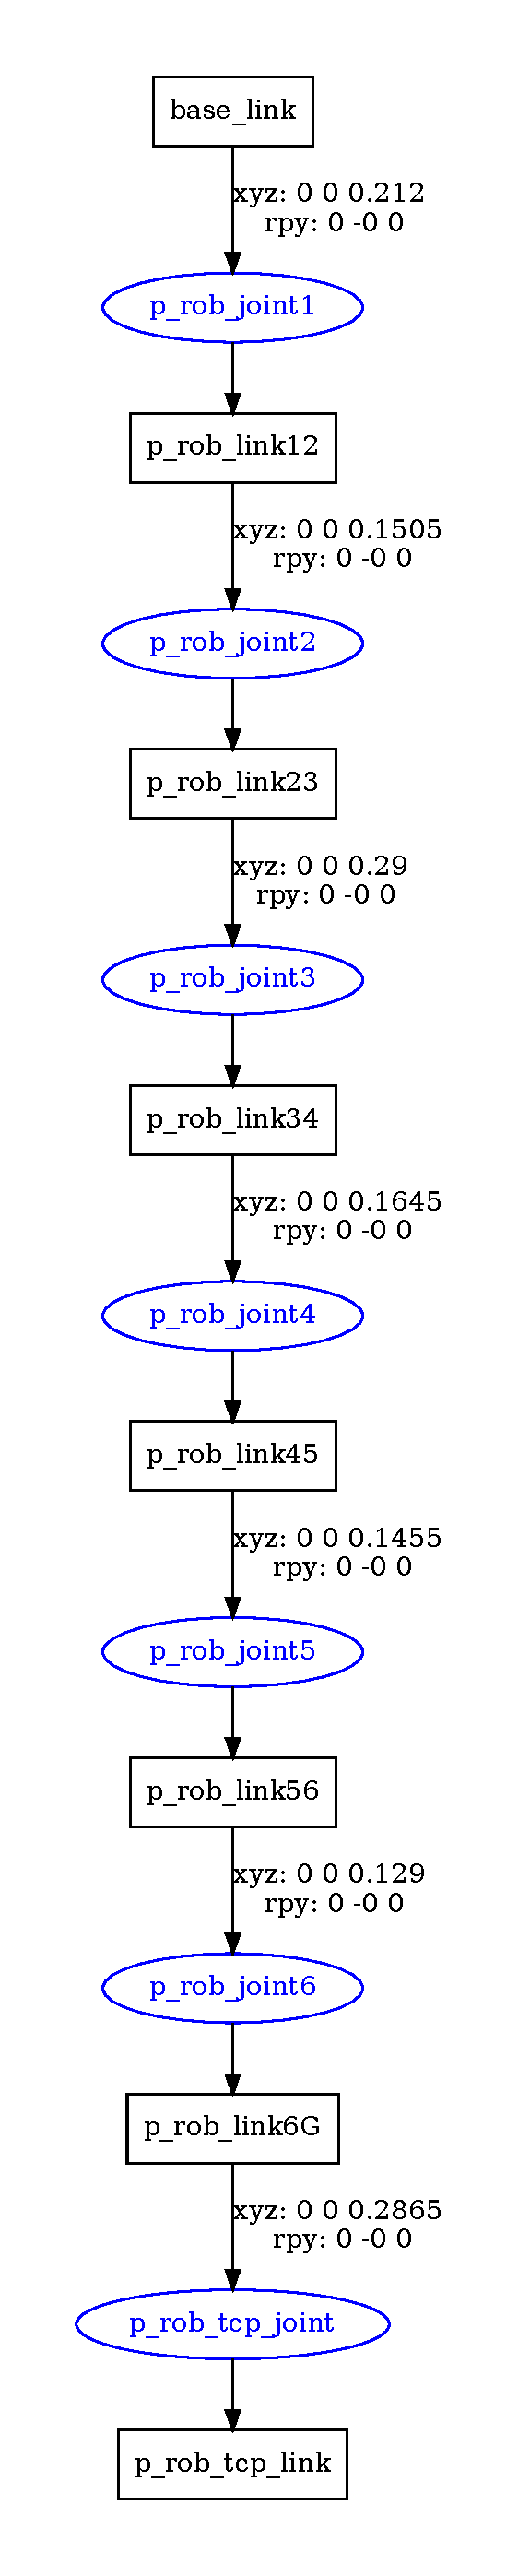
\includegraphics[width=0.3\linewidth]{./OtherFiles/p_rob.pdf}
	\caption{Catena cinematica descritta dal file urdf.}
	\label{fig:urdf_prob3}
\end{figure}
\clearpage

\todo{desrivere il metodo loadChainFromUrdf per inizializzare la libreria}

\section{Cinematica diretta e inversa}
\section{Traiettoria lineare}
\todo{Descriviamo magari qui il funzionamento base delle funzioni e poi facciamo una sezione con invece la definizione di come sono stati introdotti in star quindi plugin e componenti?}

\chapter{Implementazione in star} \todo{nome solo per far capire la sezione (es diagramma componeti)}
\section{Plugin: PluginArmPRob3Kinematics}
\section{Componente: ArmDriver e ToolInput}
